\section{手先位置制御}
\subsection{順運動学と逆運動学}

ここでは,手先位置 $(x(t), y(t))$ をその目標値 $(x^{\mathrm{ref}}(t), y^{\mathrm{ref}}(t))$ に追従させる制御を考える.

手先 $P_3$ の座標 $(x(t), y(t))$ を目標値 $(x^{\mathrm{ref}}(t), y^{\mathrm{ref}}(t))$ に追従させるためには,2.3 節で述べたように,逆運動学により角度の目標値 $\theta_x^{\mathrm{ref}}(t), \theta_y^{\mathrm{ref}}(t)$ を

\begin{equation}
\begin{cases}
\theta_x^{\mathrm{ref}}(t) = \sin^{-1} \left( \frac{\sqrt{x^{\mathrm{ref}}(t)^2 + y^{\mathrm{ref}}(t)^2}}{2\ell} \right) + \tan^{-1} \left( \frac{y^{\mathrm{ref}}(t)}{x^{\mathrm{ref}}(t)} \right) \\
\theta_y^{\mathrm{ref}}(t) = \sin^{-1} \left( \frac{\sqrt{(x^{\mathrm{ref}}(t)-2\ell)^2 + y^{\mathrm{ref}}(t)^2}}{2\ell} \right) - \tan^{-1} \left( \frac{x^{\mathrm{ref}}(t) - 2\ell}{y^{\mathrm{ref}}(t)} \right)
\end{cases}
\end{equation}

と設定すればよい.

\vspace{1em}
たとえば I--PD コントローラ(比例・微分先行型 PID コントローラ)

\begin{equation}
\begin{cases}
v_x(t) = -k_{Px} \theta_x(t) + \frac{k_{Ix}}{s} e_x(t) - k_{Dx} \frac{d\theta_x(t)}{dt} \\
v_y(t) = -k_{Py} \theta_y(t) + \frac{k_{Iy}}{s} e_y(t) - k_{Dy} \frac{d\theta_y(t)}{dt}
\end{cases}
\end{equation}

を用いると,$\theta_x(t), \theta_y(t)$ をその目標値に追従させることができ,その結果,2.2節で述べたように,順運動学により手先位置 $(x(t), y(t))$ は次式のようになる:

\begin{equation}
\begin{cases}
x(t) = h(t) \cos(\theta_x(t) - \alpha_x(t)) - \frac{d(t)}{2} \sin(\theta_x(t) - \alpha_x(t)) + \ell \sin \theta_x(t) \\
y(t) = h(t) \sin(\theta_x(t) - \alpha_x(t)) + \frac{d(t)}{2} \cos(\theta_x(t) - \alpha_x(t)) - \ell \cos \theta_x(t)
\end{cases}
\end{equation}

ただし,

\begin{equation}
\begin{cases}
d(t) = \sqrt{(p_{2x}(t) - p_{4x}(t))^2 + (p_{2y}(t) - p_{4y}(t))^2} \\
h(t) = \sqrt{\ell^2 - \left( \frac{d(t)}{2} \right)^2} \\
\alpha_x(t) = \cos^{-1} \left( \frac{\ell^2 + d(t)^2 - (p_{4x}(t)^2 + p_{4y}(t)^2)}{2\ell d} \right) \\
p_{2x}(t) = \ell \sin \theta_x(t),\quad p_{2y}(t) = -\ell \cos \theta_x(t) \\
p_{4x}(t) = 2\ell - \ell \cos \theta_y(t),\quad p_{4y}(t) = -\ell \sin \theta_y(t)
\end{cases}
\end{equation}

である.

図~\ref{fig:block_diagram} に手先位置 $(x(t), y(t))$ をその目標値 $(x^{\mathrm{ref}}(t), y^{\mathrm{ref}}(t))$ に追従させるフィードバック制御系のブロック線図を示す.

\begin{figure}[H]
  \centering
  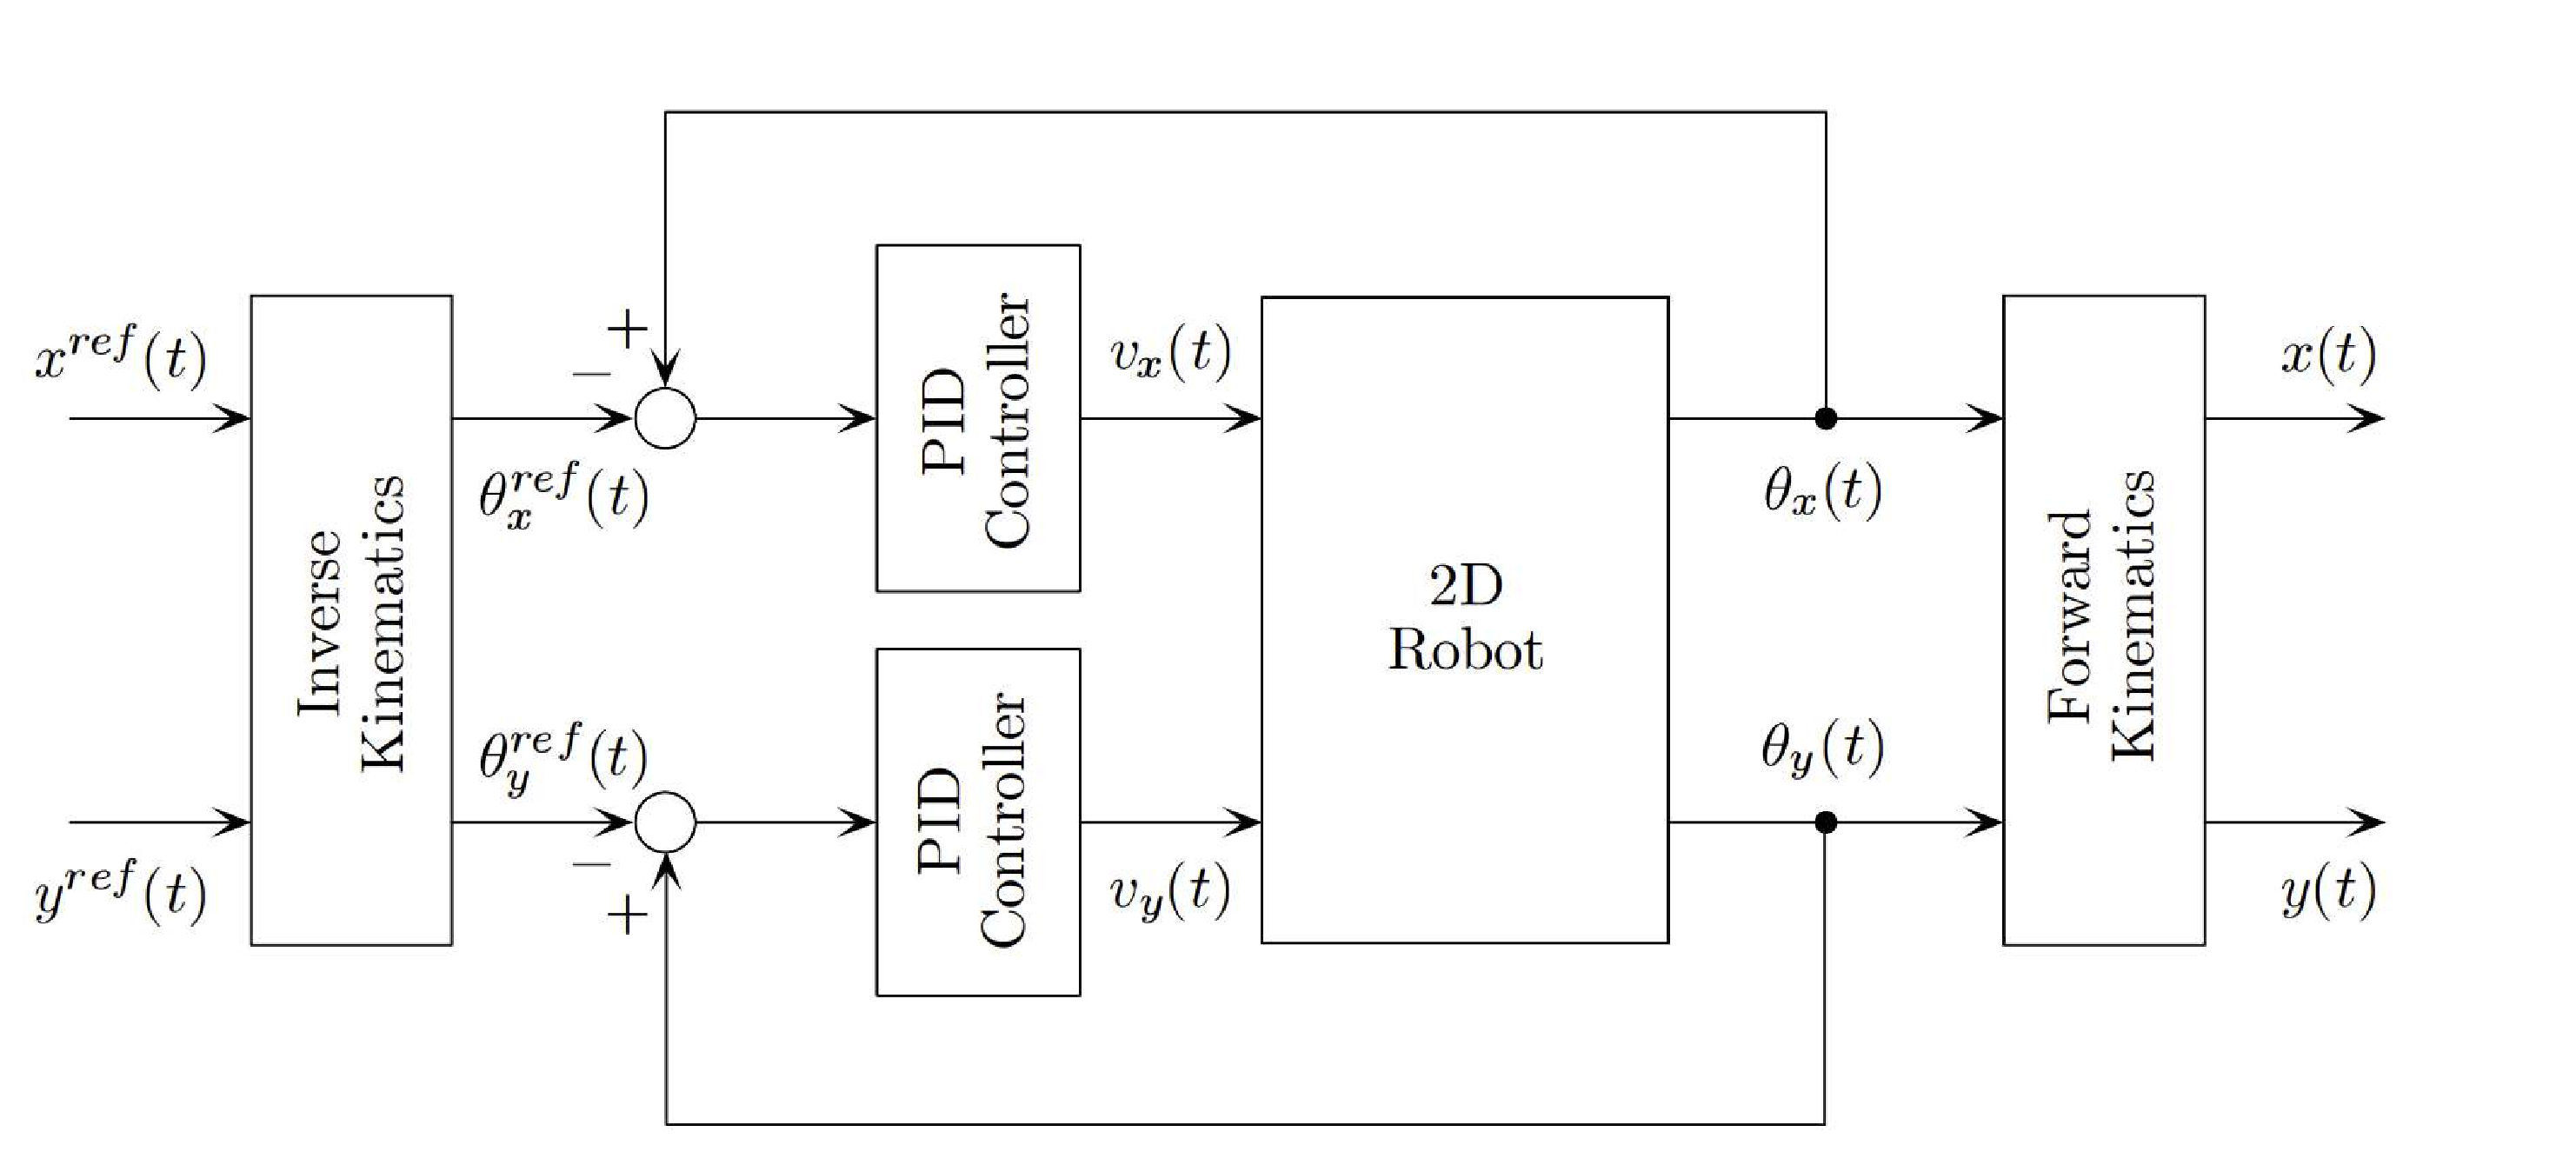
\includegraphics[width=0.85\linewidth]{figure/block6_1.pdf}
  \caption{フィードバック制御系}
  \label{fig:block_diagram}
\end{figure}

\subsection{シミュレーションと実験(目標値が一定値の場合)}

\fbox{\textbf{ステップ 1}}:
5.1.2 節で示した ``armpara.m'',5.3.2 節で示した ``armIPD.m'' およびシミュレーション結果をアニメーション表示する以下の M ファイル ``sim\_anime.m'' を作成し,\textbackslash xy に保存する.
また,シミュレーションモデル ``sim\_robot\_xy.slx''(図~\ref{fig:sim_robot_xy}(a)),実機実験モデル ``ex\_robot\_xy.slx''(図~\ref{fig:sim_robot_xy}(b))を作成し,\textbackslash xy に保存する.ただし,各 \texttt{Subsystem} の内容は以下に示すとおりである.

\begin{figure}[H]
    \centering
    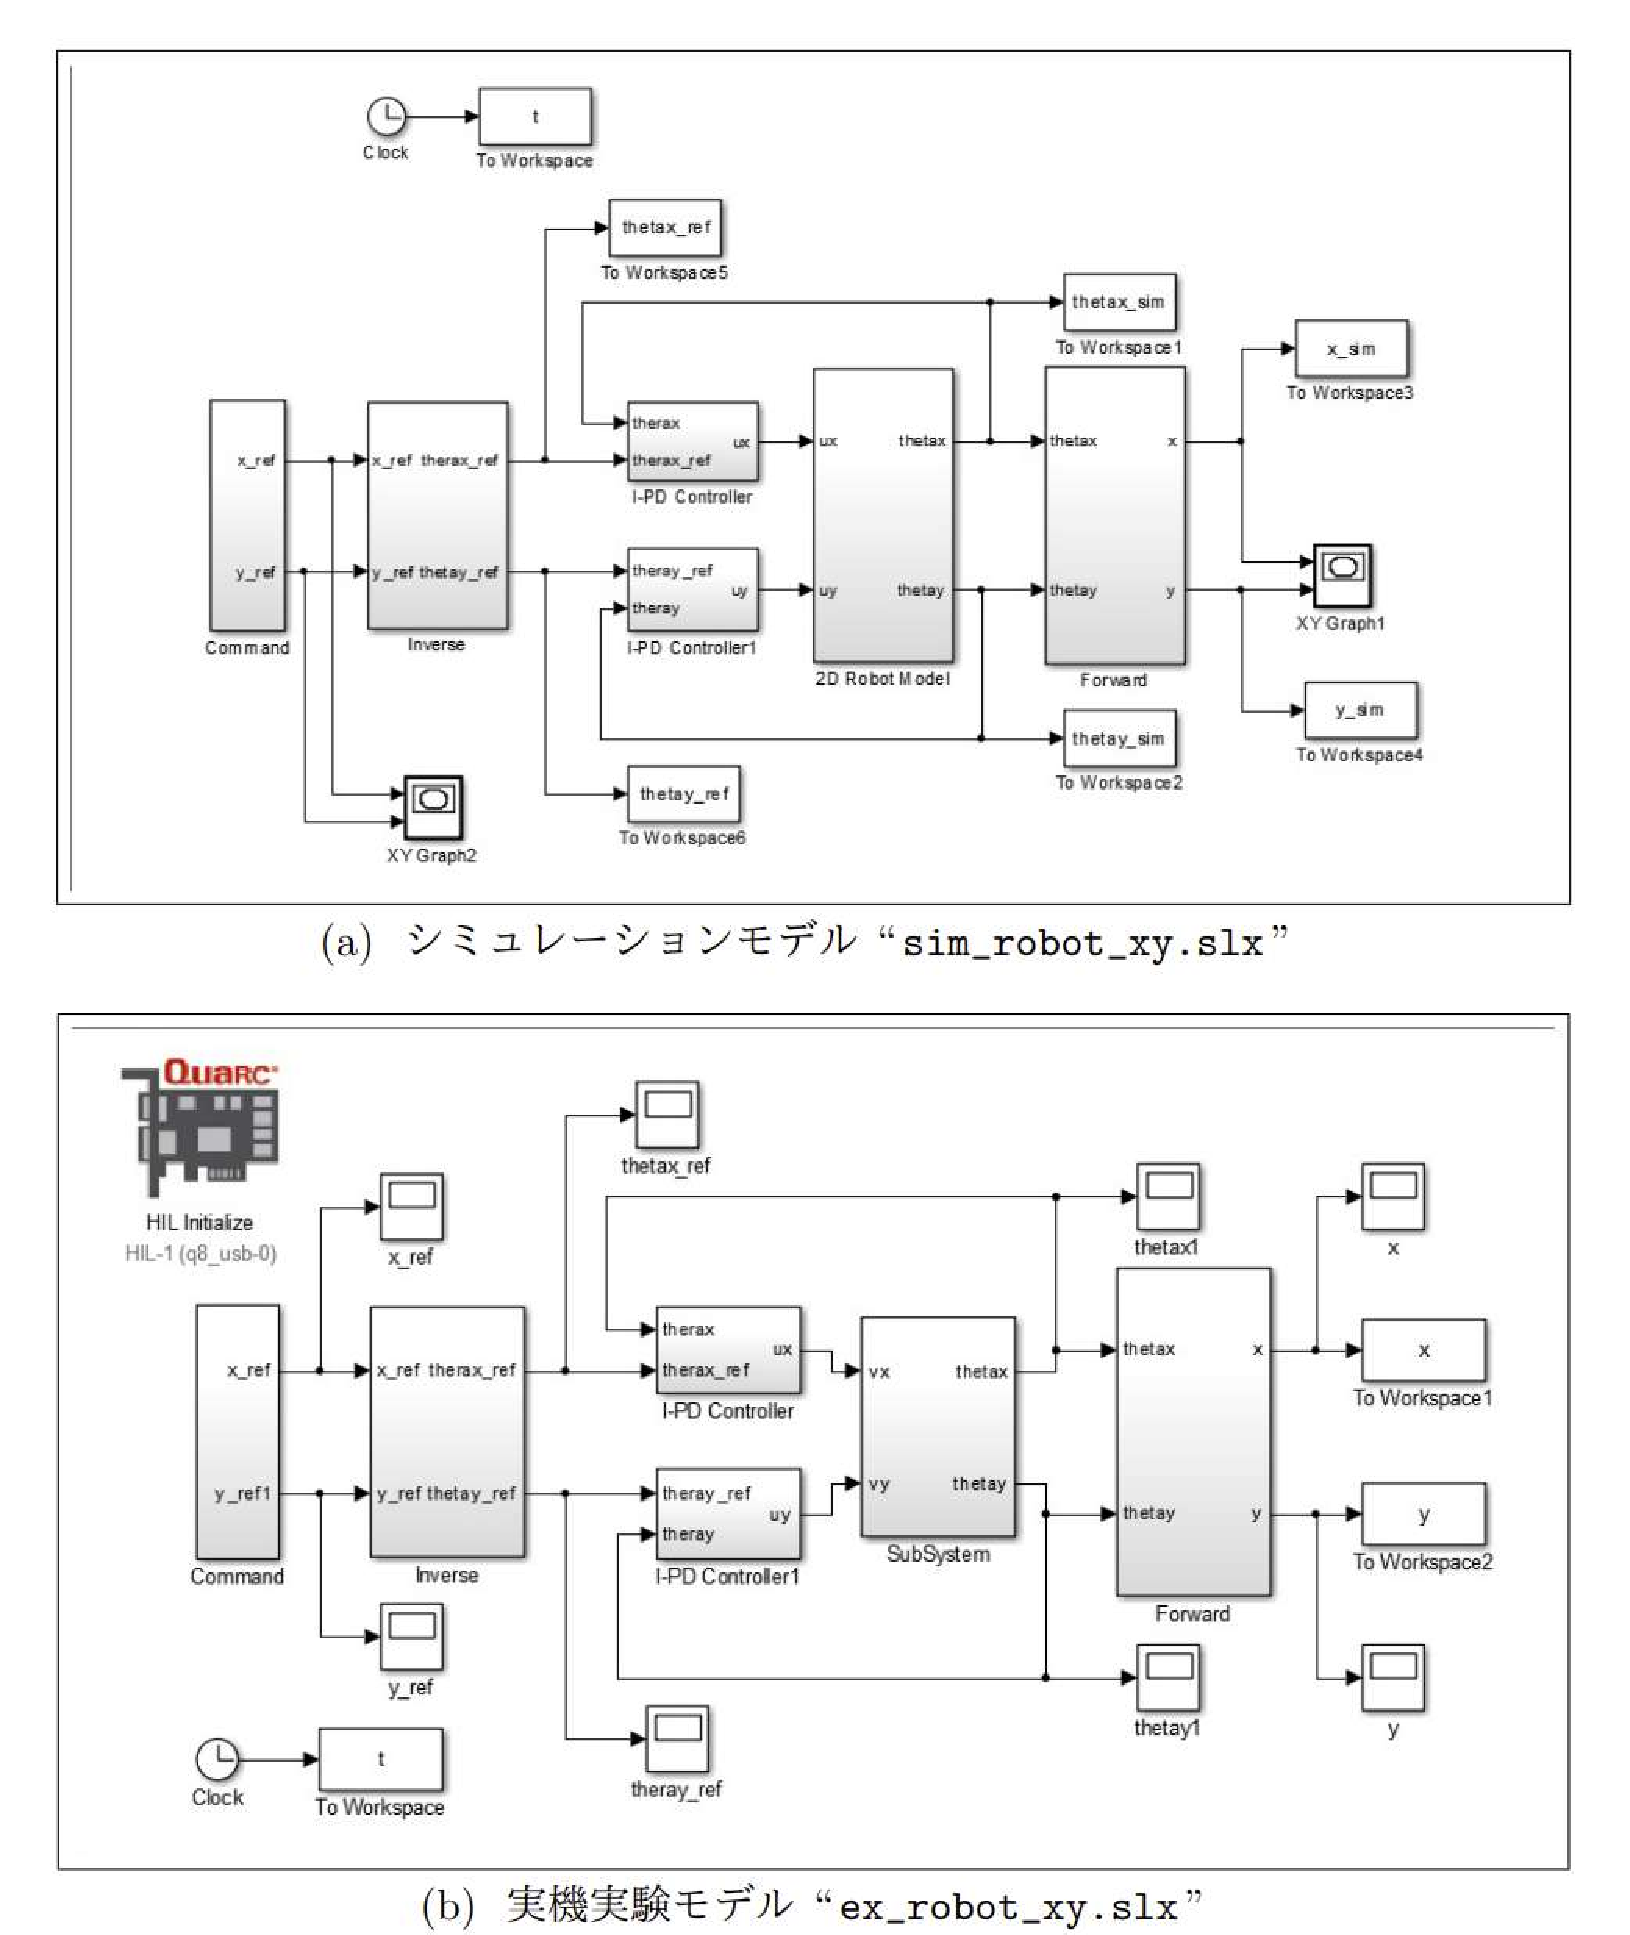
\includegraphics[width=0.85\linewidth]{figure/robot_xy_models.pdf}
    \caption{手先位置制御(目標値が一定値の場合)}
    \label{fig:sim_robot_xy}
\end{figure}

\begin{figure}[H]
    \centering
    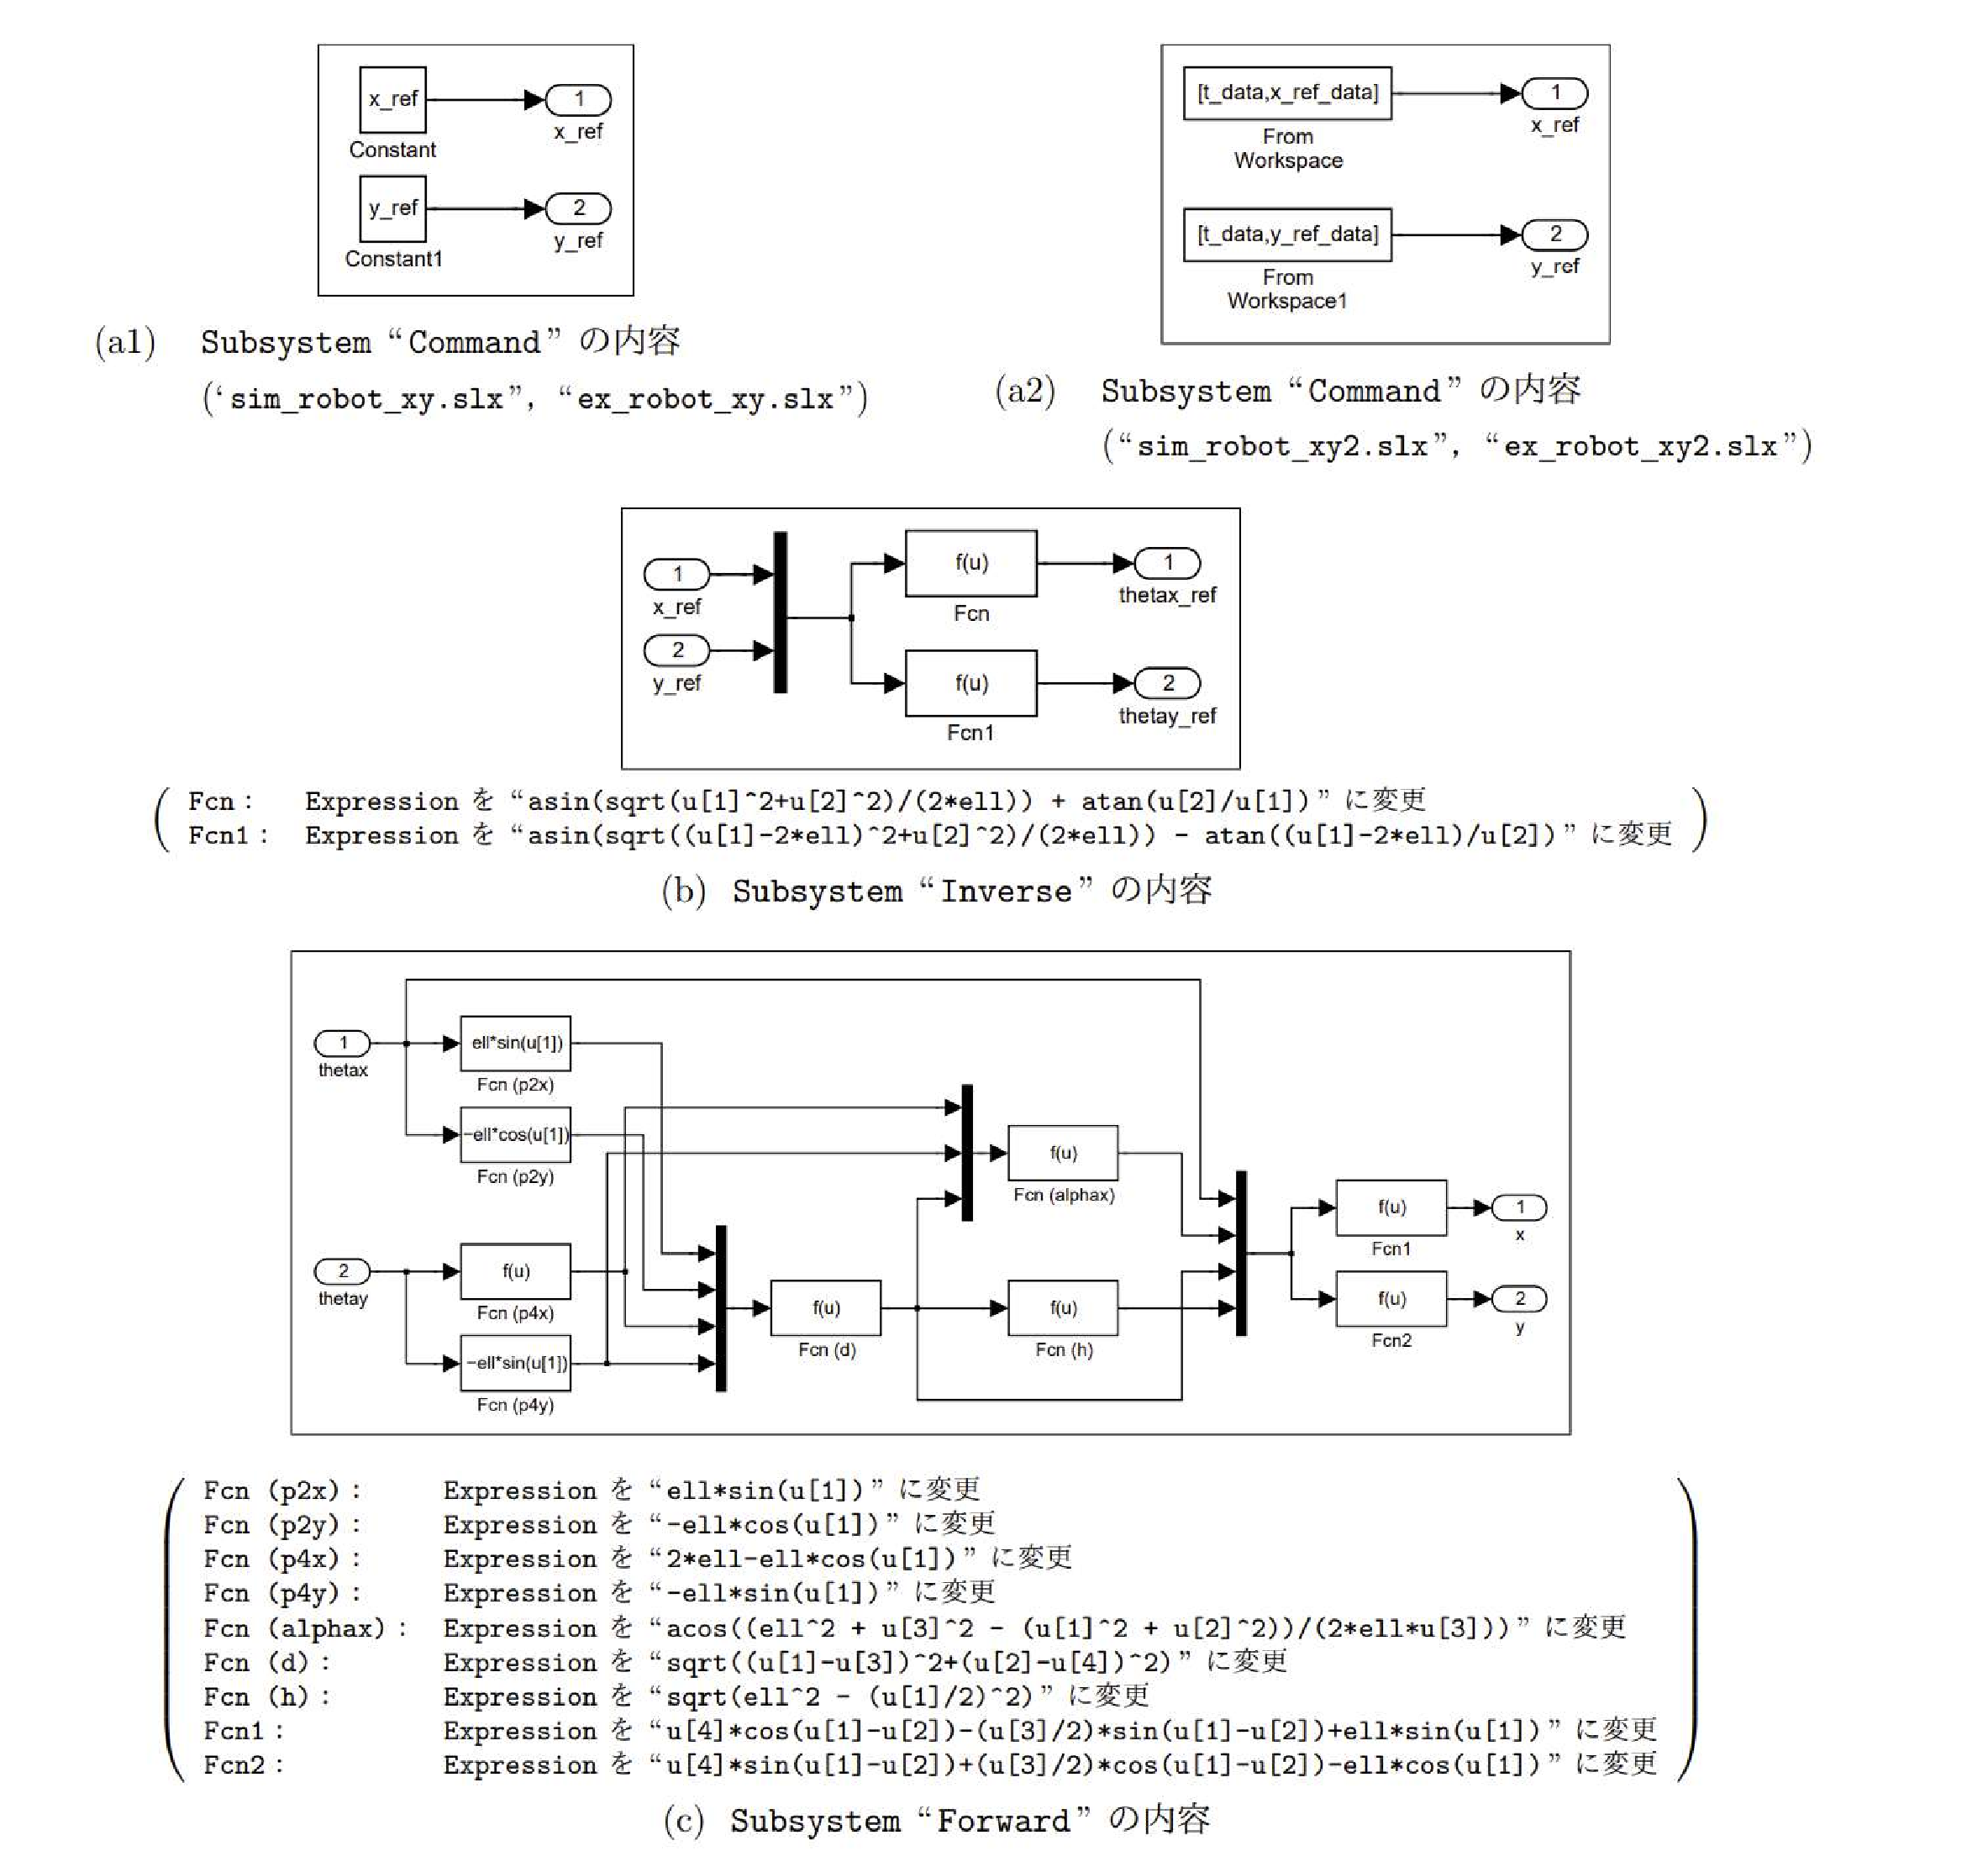
\includegraphics[width=1.0\linewidth]{figure/subsystem_all.pdf}
    \caption{Subsystem ``Command'', ``Inverse'', ``Forward'' の構成(図~6.3)}
    \label{fig:subsystems}
\end{figure}

\fbox{\textbf{ステップ 2}}: まず,MATLAB Command Window で
\begin{verbatim}
>> armIPD
各パラメータを設定して下さい
omegaMx = 20
omegaMy = 20
  …(略)…
alphaM1x = 2
alphaM2x = 2
alphaM1y = 2
alphaM2y = 2
  …(略)…
x_ref = 0.15; y_ref = -0.05;
\end{verbatim}

と入力し,パラメータを設定する.つぎに,シミュレーションを開始し,シミュレーション終了後に以下のように入力して結果をアニメーション表示する.
\begin{verbatim}
>> sim_anime;
\end{verbatim}

アニメーション(図~\ref{fig:xy_animation}~(a))によって各リンクに無理な動きがないことを確認した後,``ex\_robot\_xy.slx''をコンパイルしてから実機実験を行うと,図~\ref{fig:xy_animation}~(b) の実験結果が得られる.

\begin{figure}[H]
    \centering
    \begin{subfigure}[b]{0.45\linewidth}
        \centering
        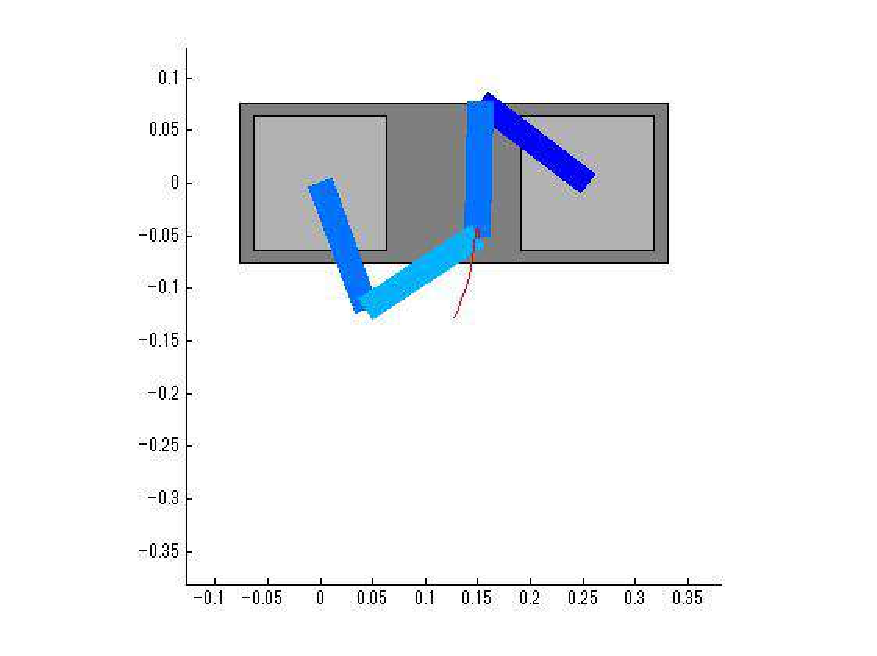
\includegraphics[width=\linewidth]{figure/sim_anime.pdf}
        \caption{シミュレーション結果のアニメーション表示}
    \end{subfigure}
    \begin{subfigure}[b]{0.45\linewidth}
        \centering
        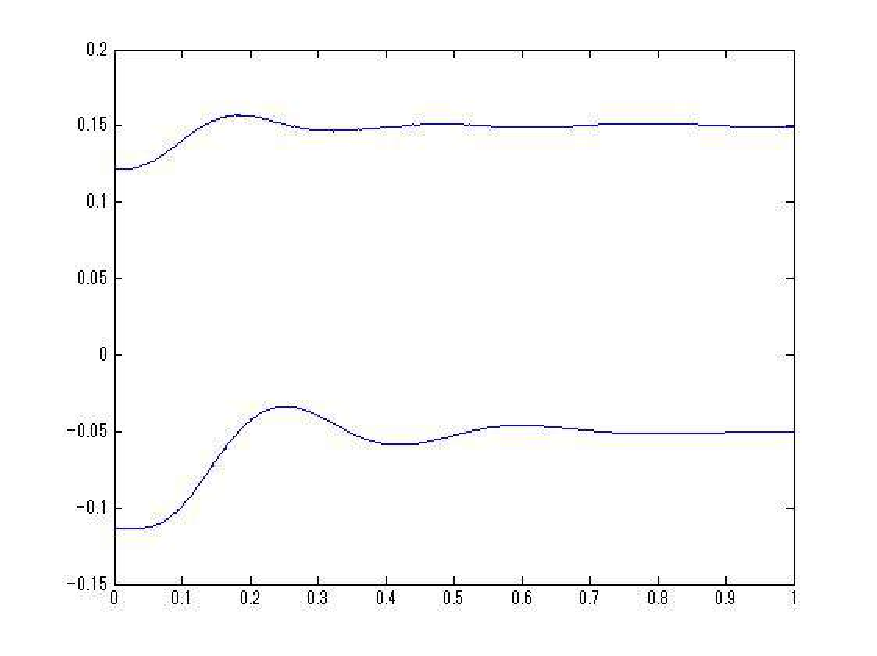
\includegraphics[width=\linewidth]{figure/ex_robot_guraf.pdf}
        \caption{実験結果}
    \end{subfigure}
    \caption{手先位置制御($x^{\mathrm{ref}}=0.15\ \mathrm{[m]}$, $y^{\mathrm{ref}}=-0.05\ \mathrm{[m]}$)}
    \label{fig:xy_animation}
\end{figure}

\subsection{シミュレーションと実験 (目標値をデータで与える場合)}
\subsubsection{目標値の与え方}
ここでは,目標値を以下のようにデータ列で与え,手先位置制御を行うことを考える.

\begin{lstlisting}[language=Matlab]
t_data       = [0; 1; 2; 3; 4];
x_ref_data   = [0.1; 0.2; 0.2; 0.1; 0.1];
y_ref_data   = [-0.15; -0.15; -0.05; -0.05; -0.15];
\end{lstlisting}

なお,このようにデータ列で目標値を与えたとき,図\ref{fig:xy_ref_data}のようになる.

\begin{figure}[H]
    \centering
    \begin{subfigure}[b]{0.45\linewidth}
        \centering
        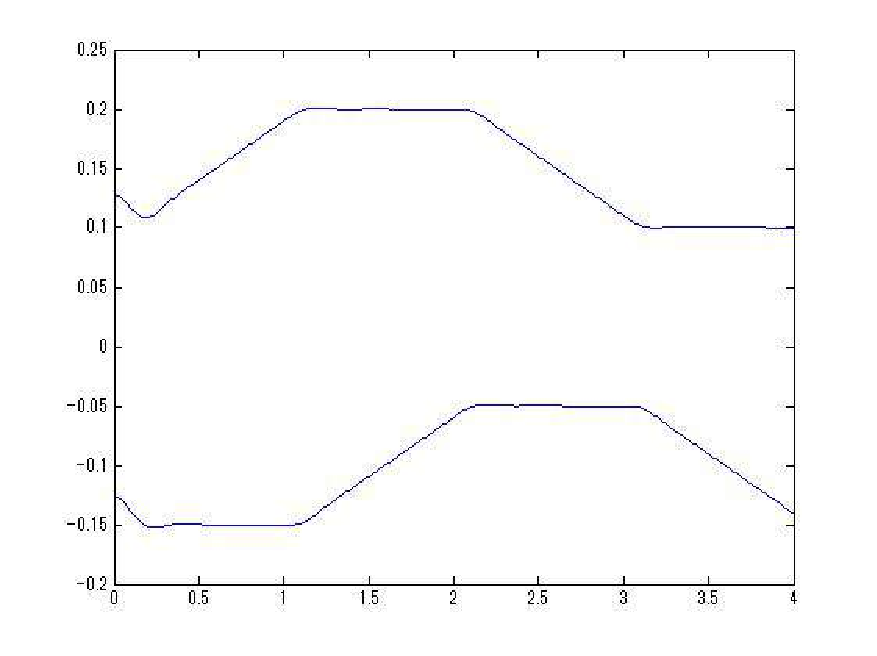
\includegraphics[width=\linewidth]{figure/sim_anime_2_grafu.pdf}
        \caption{$x^{\mathrm{ref}}(t)$ と $y^{\mathrm{ref}}(t)$}
    \end{subfigure}
    \begin{subfigure}[b]{0.45\linewidth}
        \centering
        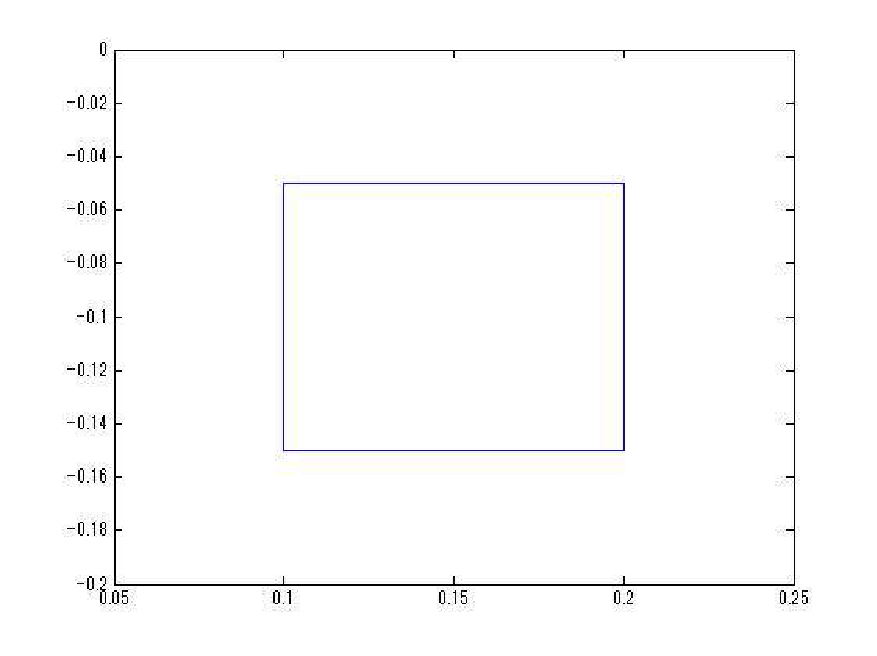
\includegraphics[width=\linewidth]{figure/sim_anime_2.pdf}
        \caption{$y^{\mathrm{ref}}$ vs $x^{\mathrm{ref}}$}
    \end{subfigure}
    \caption{データ列で与えられた手先の目標位置}
    \label{fig:xy_ref_data}
\end{figure}

\subsubsection{デモンストレーション}

ここでは,花の絵を描くような目標位置データを用いた手先位置制御のデモンストレーションを行う.
このデータは M ファイル ``flower\_data.m'' に含まれており,$(x^{\mathrm{ref}}(t), y^{\mathrm{ref}}(t))$ の時系列データとして定義されている.
この目標位置に追従する様子をアニメーション表示するために,MATLAB Command Window で以下のように入力する.

\begin{lstlisting}[language=Matlab]
flower_data                                % flower_data.m の実行(手先位置の目標値設定)
figure(1); plot(t_data,x_ref_data); 
xlabel('time [s]'); ylabel('x^{ref} [m]'); % (t, x_ref(t)) のプロット
figure(2); plot(t_data,y_ref_data); 
xlabel('time [s]'); ylabel('y^{ref} [m]'); % (t, y_ref(t)) のプロット
figure(3); plot(x_ref_data,y_ref_data);    % (x_ref(t), y_ref(t)) のプロット
xlabel('x^{ref} [m]'); ylabel('y^{ref} [m]');
t = t_data; x = x_ref_data; y = y_ref_data;
figure(4); sim_anime                       % flower_anime.m の実行(アニメーション)
\end{lstlisting}

ここでは,M ファイル ``flower\_data.m'' に含まれている花の絵のような目標位置データを用いて,手先位置制御の動作をデモンストレーションする.
このファイルには,時系列で与えられた手先の目標位置 $(x^{\mathrm{ref}}(t), y^{\mathrm{ref}}(t))$ が含まれており,それを基にアニメーション表示およびグラフ出力を行う.
MATLAB Command Window で以下のように入力すればよい.

\begin{lstlisting}[language=Matlab]
flower_data                                % flower_data.m の実行(手先位置の目標値設定)
figure(1); plot(t_data,x_ref_data); 
xlabel('time [s]'); ylabel('x^{ref} [m]'); % (t, x_ref(t)) のプロット
figure(2); plot(t_data,y_ref_data); 
xlabel('time [s]'); ylabel('y^{ref} [m]'); % (t, y_ref(t)) のプロット
figure(3); plot(x_ref_data,y_ref_data);    % (x_ref(t), y_ref(t)) のプロット
xlabel('x^{ref} [m]'); ylabel('y^{ref} [m]');
t = t_data; x = x_ref_data; y = y_ref_data;
figure(4); sim_anime                       % flower_anime.m の実行(アニメーション)
\end{lstlisting}

その結果,図\ref{fig:xy_flower} に示すような時系列グラフおよびアニメーション表示が得られる.

\begin{figure}[H]
    \centering
    \begin{subfigure}[b]{0.45\linewidth}
        \centering
        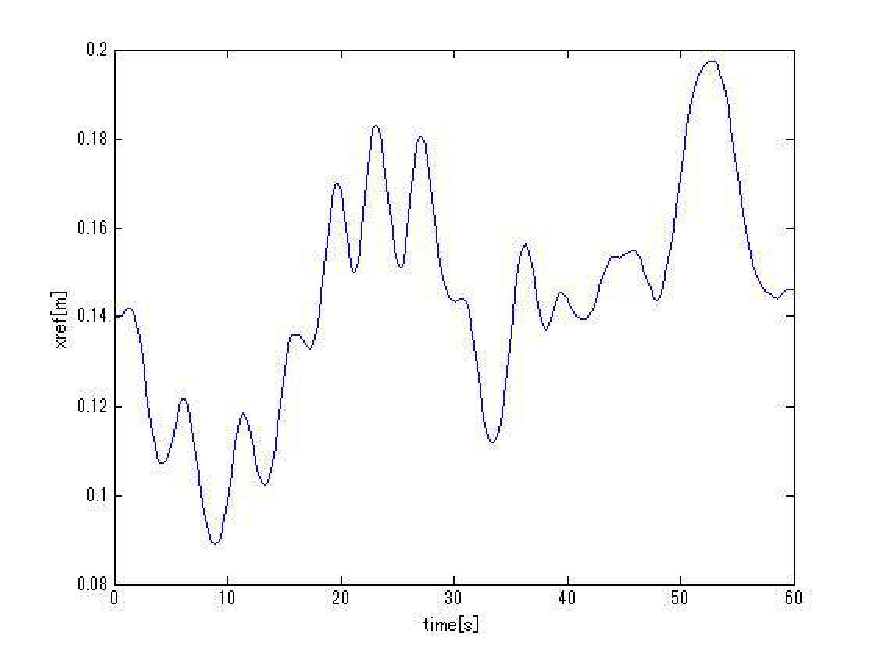
\includegraphics[width=\linewidth]{figure/xref.pdf}
        \caption{$x^{\mathrm{ref}}(t)$}
    \end{subfigure}
    \begin{subfigure}[b]{0.45\linewidth}
        \centering
        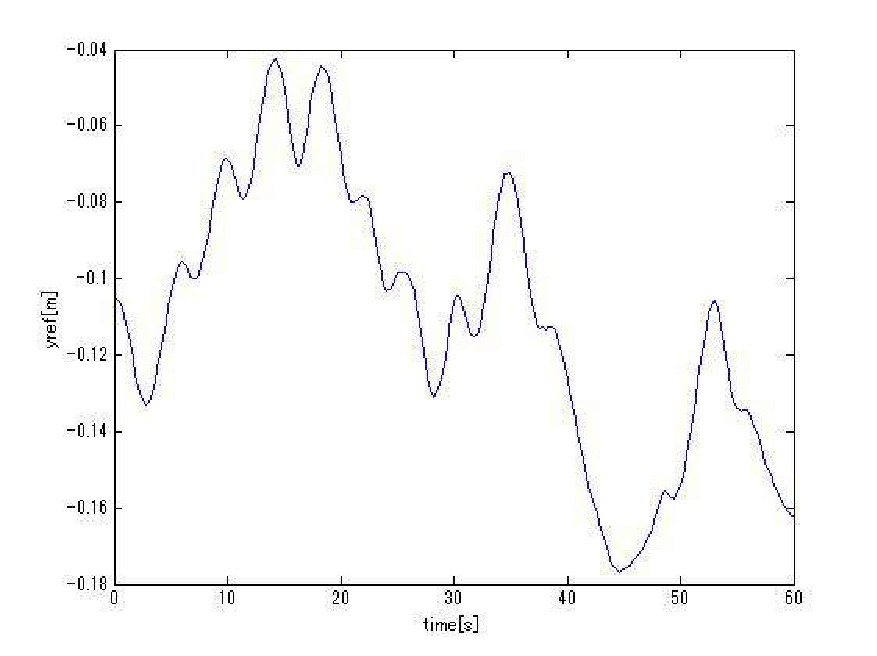
\includegraphics[width=\linewidth]{figure/yref.pdf}
        \caption{$y^{\mathrm{ref}}(t)$}
    \end{subfigure}

    \begin{subfigure}[b]{0.45\linewidth}
        \centering
        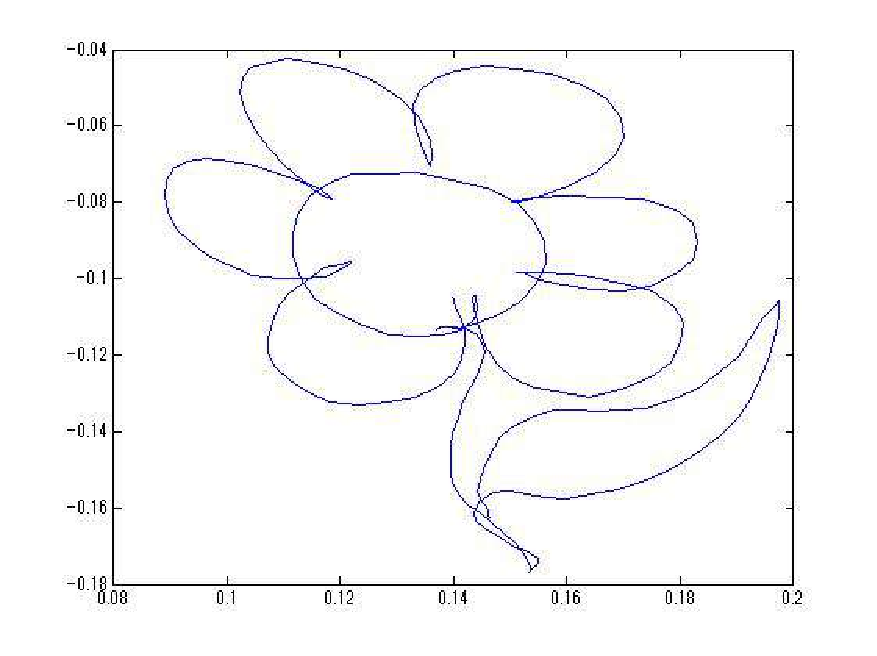
\includegraphics[width=\linewidth]{figure/mokuhyoukidou.pdf}
        \caption{目標軌道}
    \end{subfigure}
    \begin{subfigure}[b]{0.45\linewidth}
        \centering
        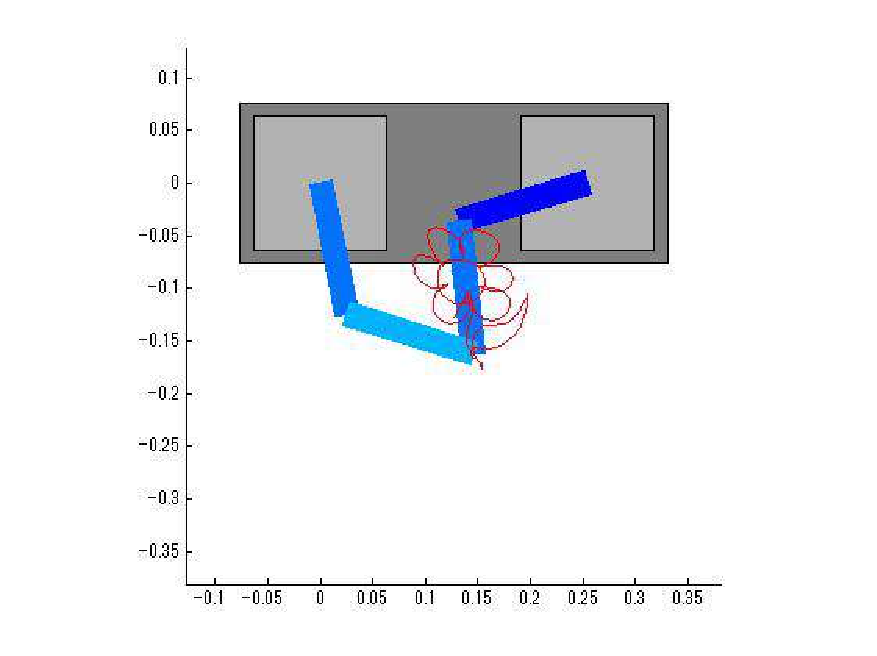
\includegraphics[width=\linewidth]{figure/fig4_sim_anime.pdf}
        \caption{アニメーション表示}
    \end{subfigure}
    \caption{\texttt{flower\_data.m} により設定された手先の目標位置}
    \label{fig:xy_flower}
\end{figure}

この花の絵の目標値データを利用して実験を行うために,MATLAB Command Window で以下のように入力
し,パラメータ設定を行う.
\begin{lstlisting}[language=Matlab]
    armIPD
    各パラメータを設定して下さい
    omegaMx = 20
    omegaMy = 20
    ........................................................... 《略》 ...........................................................
    alphaM1x = 2
    alphaM2x = 2
    alphaM1y = 2
    alphaM2y = 2
    ........................................................... 《略》 ...........................................................
    flower_data   % flower_data.m の実行(手先位置の目標値設定)
\end{lstlisting}
つぎに,``sim\_robot\_xy2.slx'' によりシミュレーションを実行する.
M ファイル \texttt{sim\_anime} を実行してアニメーションで各リンクに無理な動きがないことを確認した後,
``ex\_robot\_xy2.slx'' をコンパイルしてから実機実験を行うと,図\ref{fig:xy_flower_result} の実験結果が得られる.

\begin{figure}[H]
    \centering
    \begin{subfigure}[b]{0.45\linewidth}
        \centering
        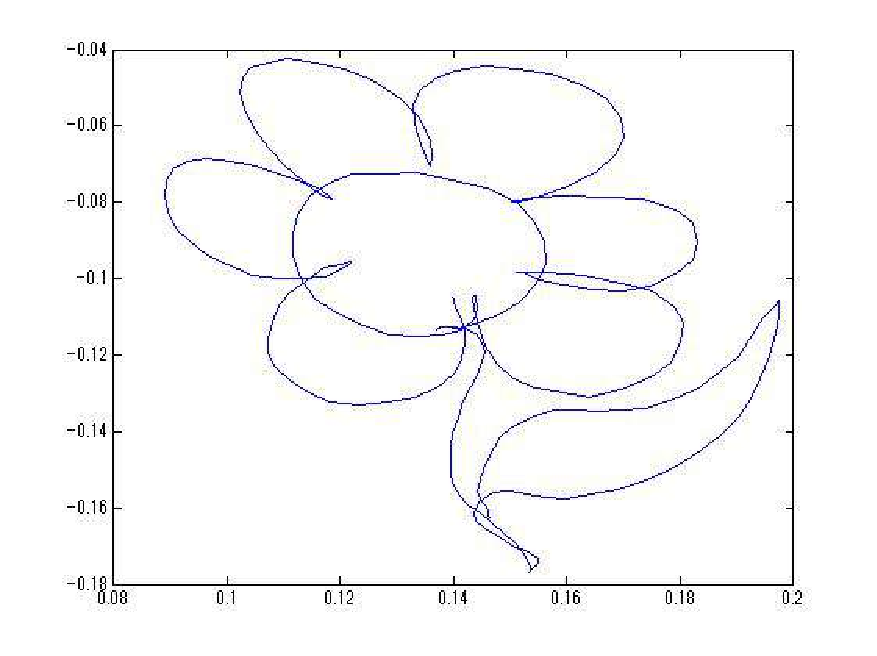
\includegraphics[width=\linewidth]{figure/mokuhyouchi.pdf}
        \caption{目標軌道}
    \end{subfigure}
    \begin{subfigure}[b]{0.45\linewidth}
        \centering
        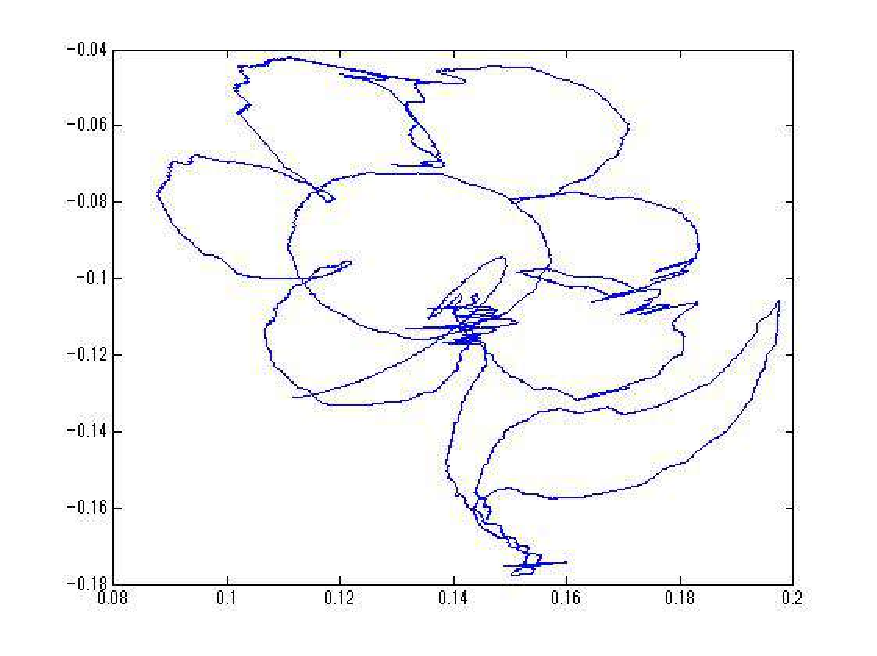
\includegraphics[width=\linewidth]{figure/zikkennkekka.pdf}
        \caption{実験結果}
    \end{subfigure}
    \caption{手先位置制御}
    \label{fig:xy_flower_result}
\end{figure}
